% (c) 2014 Daniele Masini - d.masini.it@gmail.com
\chapter{Rette parallele}

\includegraphics[width=0.95\textwidth]{intersection_de_deux_paralleles.jpg}
  \begin{center}
    {\large ``Intersection de deux parallèles''}\par
    Foto di OliBac\par
    \url{http://www.flickr.com/photos/olibac/3244014009/}\par
    Licenza: Creative Commons Attribution\par
  \end{center}
\newpage

\section{Primo teorema dell'angolo esterno}

Ricordiamo che un angolo esterno di un poligono è un angolo che ha come vertice un vertice del poligono ed è adiacente ad un angolo interno.

\begin{teorema}[dell'angolo esterno]
In un triangolo un angolo esterno è maggiore di ciascuno dei due angoli interni non adiacenti.
\end{teorema}

% figura

\begin{proof}
Sia $ABC$ un triangolo. Prolunghiamo il lato $AB$ dalla parte di $B$ e prendiamo un qualsiasi punto $D$ sul prolungamento. Vogliamo dimostrare che l'angolo $C\widehat{B}D$ è maggiore sia dell'angolo $C\widehat{A}B$ sia dell'angolo $A\widehat{C}B$. A tal fine prendiamo il punto medio del lato $CB$, lo chiamiamo $M$; uniamo $A$ con $M$ e prolunghiamo $AM$ dalla parte di $M$, prendendo un punto $N$ sul prolungamento in modo che $AM$ sia congruente a $MN$; uniamo $N$ con $B$.

Osserviamo che i triangoli $AMC$ e $BNM$ sono congruenti per il primo criterio, infatti: $CM\cong MB$ perché $M$ è un punto medio per costruzione, $AM\cong MN$ per costruzione e $C\widehat{M}A\cong B\widehat{M}N$ perché opposti al vertice.

Di conseguenza i restanti elementi dei due triangoli sono ordinatamente congruenti, in particolare $A\widehat{C}M\cong M\widehat{B}N$. Ma l'angolo $M\widehat{B}N$ è una parte propria dell'angolo esterno $C\widehat{B}D$ che risulta pertanto maggiore di $M\widehat{B}N$ e dell'angolo interno di vertice $C$.

Rimane ora da dimostrare che $C\widehat{B}D$ è anche maggiore di $C\widehat{A}B$ ma per farlo occorre un'altra costruzione.

Prolunghiamo il segmento $CB$ dalla parte di $B$ viene individuato un altro angolo esterno, che però è congruente al precedente: è anch'esso adiacente all'angolo interno di vertice $B$ ed è opposto al vertice di $C\widehat{B}D$. Usiamo tale angolo ed una costruzione analoga alla precedente a partire dal punto medio $F$ del segmento $AB$ e dal punto $G$ sul prolungamento di $CF$, con $CF\cong FG$ in modo da ottenere, dal confronto dei triangoli congruenti $AFC$ e $FGB$, che l'angolo interno di vertice $A$ è congruente all'angolo $F\widehat{B}G$ che è una parte propria dell'angolo esterno di vertice $B$.
\end{proof}

\section{Rette perpendicolari}

Ricordiamo che due rette giacenti su uno stesso piano si dicono \emph{perpendicolari} se si incontrano dividendo il piano in quattro angoli congruenti. In realtà è sufficiente sapere che uno dei quattro angoli che si vengono a formare è retto, per concludere che sono tutti retti.

\begin{proprieta}
Siano $AB$ e $CD$ due rette incidenti di intersezione $E$, se risulta che l'angolo $A\widehat{E}C$ è retto, allora sono retti anche gli angoli $A\widehat{E}D$, $B\widehat{E}C$ e $B\widehat{E}D$.
\end{proprieta}

% figura

\begin{proof}
L'angolo $A\widehat{E}D$ è retto perché adiacente a un angolo retto;
l’angolo $D\widehat{E}B$ è retto perché opposto al vertice a un angolo retto;
l’angolo $C\widehat{E}B$ è retto perché adiacente a un angolo retto.
\end{proof}

Quindi, se due rette incidenti formano un angolo retto allora tutti gli angoli che si formano sono retti

L’esistenza e l’unicità della perpendicolare sono assicurate dal seguente teorema.

\begin{teorema}
Nel piano, data una retta ed un punto, esiste ed è unica la retta perpendicolare alla retta data e passante per il punto assegnato.
\end{teorema}

% figura

\begin{proof}
Per la dimostrazione, distinguiamo due casi.

Primo caso: il punto appartiene alla retta.
Sia $AB$ una retta del piano e sia $P$ un suo punto. Allora se tracciamo la bisettrice dell'angolo piatto $A\widehat{P}B$, questa è certamente perpendicolare ad $AB$, in quanto i due angoli che si vengono a formare sono retti.
Prolungando questa bisettrice, si viene a formare una retta $CD$ perpendicolare ad $AB$.  
Supponiamo per assurdo che la retta $CD$ non sia l'unica perpendicolare ad $AB$ passante per il punto $P$ ma che ne esista un'altra. Detto $E$ un punto su tale ipotetica retta distinto da $P$, se $E$ appartenesse anche alla retta $CD$, allora $PE$ coinciderebbe con $CD$, quindi $PE$ non sarebbe distinta dalla retta $CD$; se invece $E$ non appartenesse a $CD$, unendo $E$ con $P$ si verrebbero a formare due angoli $A\widehat{P}E$ e $E\widehat{P}B$ di cui uno acuto ed uno ottuso e quindi la retta $EP$ non risulterebbe perpendicolare ad $AB$.

Secondo caso: il punto non appartiene alla retta.
Sia $AB$ una retta nel piano e sia $S$ un punto del piano non appartenente ad essa. Costruiamo la perpendicolare ad $AB$ passante per $S$ e dimostriamo che è unica.
Possiamo prendere un punto $Q$ appartenente ad $AB$ e congiungere $S$ con $Q$. Se gli angoli $A\widehat{Q}S$ e $S\widehat{Q}B$ sono retti, abbiamo già trovato la perpendicolare. Altrimenti, vuol dire che gli angoli $A\widehat{Q}S$ e $S\widehat{Q}B$ sono uno acuto ed uno ottuso. Tracciamo la semiretta $QR$, di origine $Q$ e giacente nel semipiano individuato da $AB$ non contenente il punto $S$, che divide il semipiano in due angoli, $A\widehat{Q}R$ e $R\widehat{Q}B$, rispettivamente congruenti a $A\widehat{Q}S$ e $S\widehat{Q}B$. Prendiamo un punto $T$ su tale semiretta in modo che il segmento $QT$ sia congruente a $QS$. Uniamo $S$ con $T$ e chiamiamo $H$ il punto d'intersezione tra $ST$ ed $AB$. Allora il triangolo $QTS$ è isoscele sulla base $ST$ e il segmento $QH$ è la bisettrice dell'angolo al vertice $S\widehat{Q}T$, che risulta pertanto essere anche mediana ed altezza relativa alla base $ST$. Dunque gli angoli $S\widehat{H}Q$ e $T\widehat{H}Q$ sono retti e quindi la retta $ST$ è perpendicolare ad $AB$.
Abbiamo quindi trovato la perpendicolare ad $AB$ passante per $S$. Per dimostrare che è unica possiamo ricorrere al ragionamento fatto nel primo caso, dove ora $H$ è il punto $P$ della dimostrazione precedente.
Il teorema è pertanto dimostrato.
\end{proof}

\section{Rette parallele}

Secondo la definizione di Euclide, due rette nel piano sono parallele se non hanno punti in comune.
In maniera più moderna il concetto di parallelismo è interpretato come l'avere la stessa direzione.
Si può anche dare una formulazione che unifichi le due definizioni precedenti; si deve però ricorrere al concetto di distanza: due rette nel piano sono parallele se mantengono sempre la stessa distanza. Se la distanza è nulla, le due rette sono coincidenti.
Noi utilizzeremo la seguente:
\begin{definizione}
Due rette giacenti nello stesso piano si dicono \emph{parallele} se sono coincidenti oppure non si incontrano mai.
\end{definizione}

Assumendo dunque questa come definizione di parallelismo, abbiamo bisogno di precisare il concetto di distanza.
Dati due punti $P$ e $Q$, la \emph{distanza} tra $P$ e $Q$ è la lunghezza del \emph{percorso più breve} che unisce i due punti. Questo concetto è valido anche se si riferisce alle distanze tra due città che si trovano negli stradari: sono riportate le lunghezze dei percorsi minimi tra tutte le strade alternative che collegano due città. Naturalmente, nel piano, ove si ``dispone'' di tutti i punti da poter ``attraversare'', il percorso più breve che collega due punti $P$ e $Q$ è il segmento $PQ$; quindi nella geometria euclidea assumiamo come distanza tra due punti la lunghezza del segmento avente per estremi i due punti.

Se vogliamo parlare di distanza tra due insiemi di punti, allora va considerato il percorso più breve tra tutti i percorsi che collegano un qualsiasi punto del primo insieme con un qualsiasi punto del secondo: in pratica la distanza è la lunghezza del più piccolo segmento tra tutti quelli che collegano i due insiemi di punti. 

Nel caso particolare di un punto $A$ ed una retta $BC$, se il punto appartiene alla retta allora la distanza di $A$ da $BC$ è uguale a zero, altrimenti si considera come distanza la lunghezza del segmento $AH$, dove $H$ è il punto in cui la perpendicolare a $BC$ passante per $A$ interseca la stessa retta $BC$: il motivo si intuisce in base a quanto detto, ma risulterà chiaro più avanti, quando affronteremo lo studio delle disuguaglianze tra gli elementi di un triangolo. 

Analogamente, come distanza tra due rette parallele si assume la lunghezza di un qualunque segmento che unisce il punto di una delle due rette con il piede della perpendicolare mandata da esso sull'altra retta. Affermare che tali segmenti sono tutti congruenti è un modo più preciso per dire che le due rette mantengono sempre la stessa distanza.

Ricordiamo la versione ``moderna'' del V Postulato di Euclide: \emph{dati una retta $r$ ed un punto $P$, allora esiste una ed una sola retta parallela ad $r$ e passante per $P$.}

\begin{proposizione}
Se due rette nel piano sono perpendicolari alla stessa retta, esse sono parallele tra loro.
\end{proposizione}

% figura

\begin{proof}
Sia $r$ una retta, e siano $s$ e $t$ due rette, entrambe perpendicolari ad $r$. 
Se $s$ e $t$ intersecano $r$ nello stesso punto $P$, allora per il teorema precedente necessariamente coincidono, e dunque sono parallele per la nostra definizione di parallelismo. 
Consideriamo ora il caso in cui $s$ e $t$ intersecano $r$ in due punti distinti, rispettivamente $A$ e $B$. Supponendo per assurdo che $s$ e $t$ si intersechino in un punto $C$, risulterebbero due distinte rette passanti per $C$ e perpendicolari alla stessa retta, assurdo per il teorema precedente. Dunque deve risultare $s\parallel t$.
\end{proof}

Analoghe proprietà valgono per rette parallele e per rette incidenti qualunque. Precisamente:
\begin{proposizione}
Siano date due rette parallele, se una terza retta è parallela ad una delle due, è parallela anche all'altra; inoltre, ogni retta che interseca una delle due, interseca anche l'altra.
\end{proposizione}

% figura

\begin{proof}
Siano $a$, $b$, $c$ tre rette, con $a\parallel b$. Se $a$ coincide con $b$, la tesi è banale. Supponiamo quindi che $a$ e $b$ non abbiano punti in comune.
Vogliamo dimostrare che se $c\parallel a$ allora $c\parallel b$.
La tesi è banale se $c$ coincide con $a$ oppure con $b$.
Supponiamo dunque che $c$ sia distinta da entrambe.
Dimostriamo che se $c$ non ha punti in comune con $a$, allora non può avere punti in comune neppure con $b$. Se per assurdo $c$ avesse un punto $P$ in comune con $b$, allora esisterebbero due rette distinte passanti per $P$ entrambe parallele alla stessa retta $a$, cosa che contraddice il quinto postulato di Euclide.
Dimostriamo ora che se $c$ interseca la retta $a$ allora interseca anche la retta $b$. Detto $Q$ il punto di intersezione tra le rette $a$ e $c$, se per assurdo $c$ non intersecasse la retta $b$, cioè se fosse $c\parallel b$, allora $a$ e $c$ sarebbero due rette distinte passanti per $Q$ entrambe parallele alla retta $b$, contrariamente a quanto dice il quinto postulato di Euclide.
\end{proof}

\begin{osservazione}
La proposizione precedente rappresenta una sorta di proprietà transitiva del parallelismo. In realtà si è scelto di considerare parallele sia rette nel piano che non hanno punti in comune sia rette coincidenti proprio per fare in modo che la relazione di parallelismo sia una relazione di equivalenza: riflessiva, simmetrica, transitiva. Con la definizione di parallelismo data da Euclide, al contrario, sarebbe stata solo simmetrica, ma non riflessiva né transitiva. Per convincersi della non transitività, basta considerare tre rette $a$, $b$, $c$ con $a$ e $c$ coincidenti e $b$ parallela ad entrambe e distinta da esse: allora $a\parallel b$ e $b \parallel c$, ma $a$ e $c$ non sono parallele secondo la definizione di Euclide.
\end{osservazione}

\subsection{Rette parallele tagliate da una trasversale}

Due rette parallele $a$ e $b$ vengono intersecate da una retta $c$ (detta \emph{trasversale}) che non è parallela ad esse,
\begin{itemize*}
\item se la retta $c$ è perpendicolare (ad entrambe), si vengono a formare otto angoli retti; 
\item se la retta $c$ non è perpendicolare ad esse, si vengono a formare otto angoli, di cui quattro acuti e quattro ottusi, rispetto alla posizione che occupano alle coppie vengono attribuiti i seguenti nomi:
\begin{itemize*}
\item le coppie di angoli 1 e 5, 2 e 6, 3 e 7, 4 e 8 si dicono \emph{corrispondenti} (perché occupano posizioni analoghe da una parallela all'altra);
\item le coppie di angoli 3 e 5, 4 e 6 si dicono \emph{alterni interni} (alterni perché occupano posizioni opposte rispetto alla trasversale, interni perché si trovano all'interno delle due parallele);
\item le coppie di angoli 1 e 7, 2 e 8 si dicono \emph{alterni esterni} (alterni perché sono opposti rispetto alla trasversale; esterni perché si trovano all'esterno della zona tra le due parallele);
\item le coppie di angoli 3 e 6, 4 e 5 si dicono \emph{coniugati interni} (si dicono coniugati perché stanno dalla stessa parte rispetto alla trasversale);
\item le coppie di angoli 1 e 8, 2 e 7 si dicono \emph{coniugati esterni}.
\end{itemize*}
\end{itemize*}
Inoltre le coppie 1 e 3, 2 e 4, 5 e 7, 6 e 8 sono angoli opposti al vertice.

\begin{teorema}[delle parallele {[}diretto{]}]
Se due rette tagliate da una trasversale formano una coppia di angoli alterni interni congruenti allora sono parallele.
\end{teorema}

% figura

\begin{proof}
Ragioniamo per assurdo. Supponiamo che la tesi sia falsa, cioè che le rette $a$ e $b$ non siano parallele. Se non sono parallele si incontreranno in un punto $C$. 
Allora si viene a formare il triangolo $ABC$. Per il teorema dell'angolo esterno del triangolo, l'angolo esterno $\alpha$ è maggiore dell'angolo interno $\beta$. Questa conseguenza contraddice l'ipotesi del teorema, secondo la quale gli angoli alterni interni $\alpha$ e $\beta$ sono congruenti. Allora abbiamo sbagliato a negare la tesi, che perciò risulta vera.
\end{proof}

Possiamo generalizzare il teorema precedenti ad altri casi.
\begin{teorema}[Criterio di parallelismo]
Se due rette tagliate da una trasversale danno origine ad una tra le seguenti coppie di angoli
\begin{itemize*}
\item angoli alterni interni o alterni esterni congruenti;
\item angoli corrispondenti congruenti;
\item angoli coniugati interni o coniugati esterni supplementari
\end{itemize*}
allora sono parallele.
\end{teorema}

\begin{proof}
Tenendo conto che due angoli opposti al vertice sono congruenti e due angoli adiacenti sono supplementari, se risulta che due angoli corrispondenti qualsiasi sono congruenti, allora i quattro angoli acuti sono tutti congruenti ed i quattro angoli ottusi sono congruenti, e quindi anche angoli alterni interni. Pertanto, per il teorema precedente, le rette sono parallele. Analogamente, se risultano supplementari due qualsiasi angoli coniugati (interni o esterni) risulta sempre che i quattro angoli acuti sono tutti congruenti tra loro come i quattro angoli ottusi, pertanto gli angoli alterni interni sono congruenti e, sempre per il teorema precedente, le due rette sono parallele.
\end{proof}

\begin{teorema}[delle parallele {[}inverso{]}]
Se due rette sono parallele allora esse formano con una trasversale qualsiasi due angoli alterni interni congruenti.
\end{teorema}

\begin{proof}
Dimostrazione. Ragioniamo per assurdo. Supponiamo che la tesi sia falsa, cioè che esista una coppia di angoli alterni interni $\alpha$ e $\beta$ con $\alpha>\beta$. Per il punto $P$, vertice dell'angolo $\alpha$ si potrà allora tracciare una retta $a'$ in modo che l'angolo da essa formato $\alpha'$ sia congruente a $\beta$. Ne segue che $a'$ e $b$ sono parallele perché formano angoli alterni interni congruenti. Allora esisterebbero due rette distinte, $a$ e $a'$, passanti per lo stesso punto $P$, entrambe parallele alla retta $b$. Questa conclusione contraddice il V postulato di Euclide, secondo il quale per un punto esterno a una retta passa un'unica parallela. Da questa contraddizione possiamo concludere che abbiamo sbagliato a supporre falsa la tesi, in altre parole la tesi è vera.
\end{proof}

In generale possiamo enunciare il seguente
\begin{teorema}
Se due rette sono parallele allora esse formano con una trasversale qualunque
\begin{itemize*}
\item angoli alterni interni o alterni esterni congruenti;
\item angoli corrispondenti congruenti;
\item angoli coniugati interni o coniugati esterni supplementari.
\end{itemize*}
\end{teorema}

\begin{proof}
Abbiamo già dimostrato che sono congruenti gli angoli alterni interni formati da due parallele tagliate da una trasversale. Tenendo conto che gli angoli opposti al vertice sono congruenti e gli angoli adiacenti sono supplementari, si possono dedurre facilmente tutte le tesi di questo teorema.
\end{proof}


\section{Somma degli angoli interni di un triangolo}

Passiamo ora a dimostrare il secondo teorema dell'angolo esterno di un triangolo.
\begin{teorema}
In un triangolo un angolo esterno è congruente alla somma dei due angoli interni non adiacenti.
\end{teorema}

\begin{proof}
Sia $ABC$ un triangolo e sia $C\widehat{B}D$ un angolo esterno. Tracciamo la semiretta $BE\parallel AC$ che divide l'angolo $C\widehat{B}D$ in due parti, $C\widehat{B}E$ ed $E\widehat{B}D$. L'angolo $C\widehat{B}E$ risulta congruente all'angolo $A\widehat{C}B$ in quanto i due angoli sono alterni interni rispetto alle rette parallele $AC$ e $BE$ tagliate dalla trasversale $CB$; analogamente l'angolo $E\widehat{B}D$ risulta congruente all'angolo $C\widehat{A}B$ in quanto i due angoli sono corrispondenti rispetto alle rette parallele $AC$ e $BE$ tagliate dalla trasversale $AD$. Dunque $C\widehat{B}D$ è congruente alla somma degli angoli interni di vertici $A$ e $C$.
\end{proof}

\begin{corollario}
La somma degli angoli interni di un triangolo è congruente ad un angolo piatto.
\end{corollario}
\begin{proof}
Dalla figura precedente $A\widehat{B}D\cong A\widehat{B}C + C\widehat{B}E + E\widehat{B}D\cong A\widehat{B}C + B\widehat{C}A + C\widehat{A}B$, pertanto la somma degli angoli interni è congruente all'angolo piatto $A\widehat{B}D$.
\end{proof}
\begin{corollario}
Un triangolo non può avere più di un angolo retto e/o ottuso.
\end{corollario}
Dunque, necessariamente almeno due angoli sono acuti. Di conseguenza, gli angoli alla base di un triangolo isoscele devono essere acuti.

\subsection{Somma degli angoli interni di un poligono}

\begin{teorema}
Dato un poligono $P$ di $n$ lati, la somma degli angoli interni di $P$ è $(n – 2)$ angoli piatti.
\end{teorema}
\begin{proof}
Infatti, dato un qualunque poligono (anche concavo) di $n$ lati, scelto un opportuno punto interno in modo che, congiunto con ciascun vertice, il poligono resti diviso in $n$ triangoli, si può osservare che la somma degli angoli interni del poligono è data dalla somma degli angoli interni di $n$ triangoli meno l'angolo giro al centro, in figura l'angolo $J$.
\end{proof}

\begin{teorema}
La somma degli angoli esterni di un qualsiasi poligono convesso, indipendentemente dal numero dei lati, è congruente ad un angolo giro.
\end{teorema}
\begin{proof}
Ogni angolo esterno è adiacente ad un angolo interno, per cui se si hanno $m$ lati e quindi $m$ vertici la somma degli angoli interni e degli angoli esterni è pari ad $m$ angoli piatti; essendo $(m – 2)$ angoli piatti la somma degli angoli interni, sarà di due angoli piatti (quindi un angolo giro) la somma degli angoli esterni.
\end{proof}


\section{Generalizzazione dei criteri di congruenza dei triangoli}

Se due triangoli hanno rispettivamente due angoli congruenti, allora anche i terzi angoli saranno congruenti nei due triangoli, in quanto supplementari della somma di angoli congruenti.

Dunque, se due triangoli hanno congruenti un lato e due angoli, anche se il lato congruente non è compreso tra i due angoli congruenti, risultano congruenti. Precisamente, vale la seguente proposizione.

\begin{teorema}[2\textsuperscript{o} Criterio di congruenza generalizzato]
Due triangoli sono congruenti se hanno rispettivamente congruenti una coppia di lati e due coppie di angoli ugualmente posti rispetto ai lati congruenti.
\end{teorema}

\begin{proof}
Il caso in cui il lato congruente è compreso tra gli angoli congruenti è stato già esaminato ed utilizzato per la dimostrazione di varie proprietà. Ora esaminiamo l'altro caso.

In figura abbiamo rappresentato due triangoli, $ABC$ e $DEF$ che hanno per ipotesi i lati $AC\cong DF$ e gli angoli $B\widehat{A}C\cong E\widehat{D}F$ e $A\widehat{B}C\cong D\widehat{E}F$. I due triangoli risultano congruenti.

La tesi segue dal fatto che deve risultare $B\widehat{A}C\cong E\widehat{F}D$, in quanto tali angoli sono supplementari alla somma di angoli congruenti per ipotesi. Ci si riconduce quindi al caso del secondo criterio di congruenza già dimostrato in precedenza.
\end{proof}

Riprendiamo una proprietà dei triangoli isosceli che abbiamo enunciato ma non abbiamo dimostrato:
\begin{proposizione}
In un triangolo isoscele l'altezza relativa alla base è anche bisettrice dell'angolo al vertice e mediana relativa alla base.
\end{proposizione}

\noindent Ipotesi: $IG\cong IH$, $I\widehat{G}H\cong I\widehat{H}G$, $IL\perp GH$.\tab Tesi: $G\widehat{I}L\cong H\widehat{I}L$, $GL\cong LH$.

\begin{proof}
I triangoli $GLI$ e $LHI$ sono congruenti per il secondo criterio generalizzato, avendo congruenti un lato e due angoli. Di conseguenza, i restanti elementi sono ordinatamente congruenti, in particolare $GL\cong LH$ e $G\widehat{I}L\cong H\widehat{I}L$.
\end{proof}

\begin{osservazione}
Dall'esame dei primi tre criteri di congruenza dei triangoli, nonché dalla generalizzazione del secondo criterio, si potrebbe essere indotti a pensare che due triangoli sono congruenti se hanno tre coppie di elementi rispettivamente congruenti, se almeno una delle tre coppie di elementi è costituita da lati.
In realtà, il primo criterio non si può generalizzare come il secondo. Basta pensare alla figura seguente: $ADC$ è un triangolo isoscele, $B$ è un punto sul prolungamento della base $AD$. Unendo $B$ con $C$, vengono individuati due nuovi triangoli, $ABC$ e $DBC$ che hanno in comune il lato $CB$ e l'angolo di vertice $B$, ed hanno inoltre congruenti i lati $AC$ e $CD$, ma evidentemente non sono congruenti. Quindi se due triangoli hanno due lati ed un angolo qualsiasi congruenti, non è detto che siano congruenti. Però nei due triangoli citati in figura, gli angoli $C\widehat{A}B$ e $C\widehat{D}B$ sono supplementari.
\end{osservazione}

Tale osservazione fa da premessa al quarto criterio di congruenza dei triangoli.
\begin{teorema}[4\textsuperscript{o} criterio di congruenza dei triangoli]
Due triangoli sono congruenti se hanno congruenti due coppie di lati e l'angolo opposto ad uno di essi, a patto che l'angolo opposto all'altra coppia di lati congruenti sia della stessa specie (cioè sia, in entrambi i triangoli, acuto oppure retto oppure ottuso).
\end{teorema}

\noindent Ipotesi: $AC\cong DF$, $CB\cong FE$, $C\widehat{A}B\cong F\widehat{D}E$, $C\widehat{B}A\cong F\widehat{E}D$.\tab Tesi: $ABC\cong DEF$.

\begin{proof}
Sulla semiretta $AB$ prendiamo il punto $G$ in maniera tale che $AG$ sia congruente a $DE$. I triangoli $AGC$ e $DEF$ saranno congruenti per il primo criterio, poiché $AC\cong DF$ e $C\widehat{A}B\cong F\widehat{D}E$ per ipotesi, $AG\cong DE$ per costruzione. Di conseguenza anche i rimanenti elementi risulteranno congruenti, in particolare $CG\cong FE$ e $C\widehat{G}A\cong F\widehat{E}D$.

Se il punto $G$ coincide con $B$, abbiamo dimostrato la congruenza dei triangoli $ABC$ e $DEF$. Altrimenti, il segmento $CG$, dovendo essere congruente ad $FE$, risulta congruente a $CB$. Dunque il triangolo $CGB$ è isoscele sulla base $GB$. Gli angoli alla base $C\widehat{G}B$ e $C\widehat{B}G$, congruenti, sono necessariamente acuti. Distinguiamo due casi:
\begin{itemize*}
\item se $G$ è interno al segmento $AB$, $C\widehat{G}B$ è esterno al triangolo $AGC$ e $C\widehat{B}G$ è interno al triangolo $ABC$, quindi $D\widehat{E}F\cong A\widehat{G}C$ ottuso e $A\widehat{B}C$ acuto;
\item se $G$ è esterno al segmento $AB$, $C\widehat{G}B$ è interno al triangolo $AGC$ e $C\widehat{B}G$ è esterno al triangolo $ABC$, quindi $D\widehat{E}F\cong A\widehat{G}C$ acuto e $A\widehat{B}C$ ottuso.
\end{itemize*}
Dunque, in nessuno dei due casi viene rispettata l'ipotesi: sono della stessa specie.
\end{proof}

\subsection{Congruenze di triangoli rettangoli}

Per quanto affermato nelle proposizioni precedenti, sappiamo che i triangoli rettangoli hanno una coppia di angoli congruenti (quelli retti, essendo tutti congruenti fra loro, come affermato dal IV postulato di Euclide) e gli altri angoli necessariamente acuti, in quanto la somma degli angoli interni di un triangolo è congruente ad un angolo piatto (come segue dal secondo teorema dell'angolo esterno e dai corollari).

Tenendo conto dunque dei criteri di congruenza dei triangoli, si possono riformulare dei criteri di congruenza specifici per i triangoli rettangoli.


%\newpage

%% (c) 2014 Daniele Masini - d.masini.it@gmail.com
\section{Esercizi}

\begin{esercizio}
\label{ese:2.1}
In base alla figura a lato rispondi alle seguenti domande\\
\begin{minipage}{.7\linewidth}
\begin{enumeratea}
\item Il lato $AB$ si oppone all'angolo \ldots\ldots\ldots
\item L'angolo $\alpha$ si oppone al lato \ldots\ldots\ldots
\item L'angolo di vertice $C$ si chiama \ldots\ldots\ldots
\item L'angolo $\gamma$ è adiacente ai lati \ldots\ldots{} e \ldots\ldots
\item I lati $AB$ e $BC$ sono adiacenti all'angolo \ldots\ldots
\item I lati $AC$ e $AB$ formano l'angolo \ldots\ldots
\item Traccia l'angolo esterno al triangolo nel vertice $A$
\item Traccia la bisettrice dell'angolo $\beta$
\item Traccia l'altezza relativa alla base $AB$
\item Traccia la mediana relativa al lato $BC$
\end{enumeratea}
\end{minipage}\hfil
\begin{minipage}{.3\linewidth}
%\begin{wrapfigure}{r}{0pt}
  \centering
    % Copyright (c) 2015 Daniele Masini - d.masini.it@gmail.com

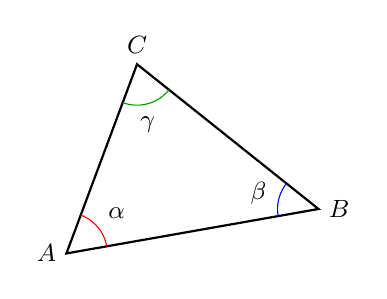
\begin{tikzpicture}[scale=1.3,font=\small]
\usetikzlibrary{calc}

\begin{scope}[rotate=10]
\coordinate (a) at (0,0);
\coordinate (c) at (1,1.7);
\coordinate (b) at (2.5,0);

\draw[thick] (b) node[right] {$B$} -- (c) node[above] {$C$} -- (a) node[left] {$A$} -- cycle;

\begin{scope}
\clip (a) -- (b) -- (c) -- cycle;
\draw[red] (a) circle (0.4);
\node at ([shift={(.55,.3)}]a) {$\alpha$};
\draw[blue] (b) circle (0.4);
\node at ([shift={(-.55,.25)}]b) {$\beta$};
\draw[green!60!black] (c) circle (0.4);
\node at ([shift={(0,-.6)}]c) {$\gamma$};
\end{scope}

\end{scope}

\end{tikzpicture}

%\end{wrapfigure}
\end{minipage}
\end{esercizio}

\begin{esercizio}
\label{ese:2.2}
Disegna un segmento $AB$, quindi disegna i triangoli $ABC$ e $ABD$ che hanno la base $AB$ in comune.
\end{esercizio}

\begin{esercizio}
\label{ese:2.3}
Disegna le tre altezze di ciascuno dei triangoli nella figura~\ref{fig:ese2.3}.
\end{esercizio}

\begin{figure}[htb]
\centering% Copyright (c) 2015 Daniele Masini - d.masini.it@gmail.com

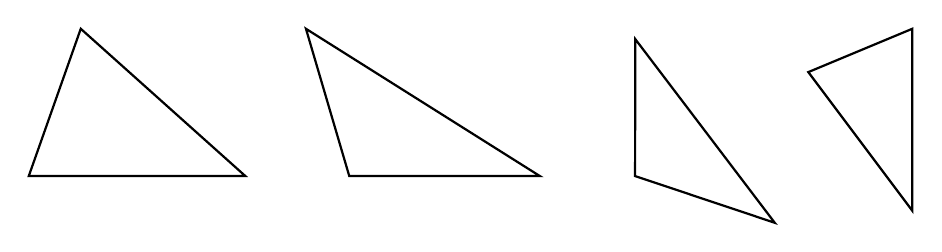
\begin{tikzpicture}[scale=1.1,font=\small]
\usetikzlibrary{calc}

\begin{scope}
\coordinate (a) at (0,0);
\coordinate (c) at (0.6,1.7);
\coordinate (b) at (2.5,0);
\draw[thick] (b)-- (c) -- (a) -- cycle;
\end{scope}

\begin{scope}[xshift=3.7cm]
\coordinate (a) at (0,0);
\coordinate (c) at (-.5,1.7);
\coordinate (b) at (2.2,0);
\draw[thick] (b)-- (c) -- (a) -- cycle;
\end{scope}

\begin{scope}[xshift=7cm, rotate=-18.5]
\coordinate (a) at (0,0);
\coordinate (c) at (-.5,1.5);
\coordinate (b) at (1.7,0);
\draw[thick] (b)-- (c) -- (a) -- cycle;
\end{scope}

\begin{scope}[xshift=9cm]
\coordinate (a) at (0,1.2);
\coordinate (c) at (1.2,1.7);
\coordinate (b) at (1.2,-0.4);
\draw[thick] (b)-- (c) -- (a) -- cycle;
\end{scope}


\end{tikzpicture}

\caption{Esercizio~\ref{ese:2.3}}\label{fig:ese2.3}
\end{figure}

\begin{esercizio}
\label{ese:2.4}
Per ciascuna delle coppie di triangoli a lato indica se sono congruenti ed eventualmente per quale criterio.\\
\begin{minipage}{.5\linewidth}
\begin{enumeratea}
\item Si sa che sono congruenti i lati $AB$ con $A'B'$ e $AC$ con $A'C'$, l'angolo $\widehat{A}$ con l'angolo $\widehat{A'}$.\\
I triangoli sono congruenti?\tab	Sì\quad	No\\
Se sì, per il \ldots\ldots\ldots\ldots\ldots\ldots\ldots\ldots

\item Si sa che sono congruenti i lati $AB$ con $A'B'$ e gli angoli $\widehat{A}$ con $\widehat{B'}$ e $\widehat{B}$ con $\widehat{A'}$.\\
I triangoli sono congruenti?\tab	Sì\quad	No\\
Se sì, per il \ldots\ldots\ldots\ldots\ldots\ldots\ldots\ldots

\item Si sa che sono congruenti i lati $AB$ con $A'B'$ e $BC$ con $A'C'$, l'angolo $\widehat{A}$ con $\widehat{A'}$.\\
I triangoli sono congruenti?\tab	Sì\quad	No\\
Se sì, per il \ldots\ldots\ldots\ldots\ldots\ldots\ldots\ldots
\end{enumeratea}
\end{minipage}\hfil
\begin{minipage}{.4\linewidth}
  \centering
    % Copyright (c) 2015 Daniele Masini - d.masini.it@gmail.com

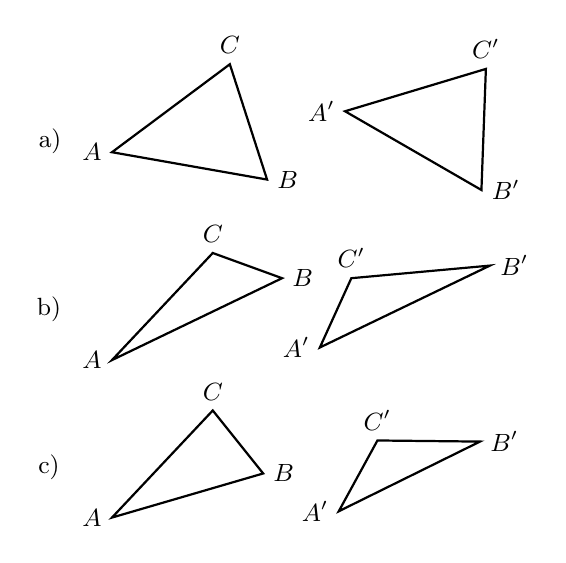
\begin{tikzpicture}[scale=0.8,font=\small]
\usetikzlibrary{calc}

\begin{scope}[rotate=-10]
\coordinate (a) at (0,0);
\coordinate (c) at (1.6,1.7);
\coordinate (b) at (2.5,0);
\draw[thick] (b) node[right] {$B$} -- (c) node[above] {$C$} -- (a) node[left] {$A$} -- cycle;
\node at (-1,0) {a)};
\end{scope}

\begin{scope}[xshift=3.7cm,yshift=0.65cm,rotate=-30]
\coordinate (a) at (0,0);
\coordinate (c) at (1.6,1.7);
\coordinate (b) at (2.5,0);
\draw[thick] (b) node[right] {$B'$} -- (c) node[above] {$C'$} -- (a) node[left] {$A'$} -- cycle;
\end{scope}

\begin{scope}[yshift=-3.3cm]
\coordinate (a) at (0,0);
\coordinate (c) at (1.6,1.7);
\coordinate (b) at (2.7,1.3);
\draw[thick] (b) node[right] {$B$} -- (c) node[above] {$C$} -- (a) node[left] {$A$} -- cycle;
\node at (-1,0.8) {b)};
\end{scope}

\begin{scope}[xshift=3.3cm,yshift=-3.1cm]
\coordinate (a) at (0,0);
\coordinate (c) at (0.5,1.1);
\coordinate (b) at (2.7,1.3);
\draw[thick] (b) node[right] {$B'$} -- (c) node[above] {$C'$} -- (a) node[left] {$A'$} -- cycle;
\end{scope}

\begin{scope}[yshift=-5.8cm]
\coordinate (a) at (0,0);
\coordinate (c) at (1.6,1.7);
\coordinate (b) at (2.4,0.7);
\draw[thick] (b) node[right] {$B$} -- (c) node[above] {$C$} -- (a) node[left] {$A$} -- cycle;
\node at (-1,0.8) {c)};
\end{scope}

\begin{scope}[xshift=3.6cm,yshift=-5.7cm,rotate=10]
\coordinate (a) at (0,0);
\coordinate (c) at (0.8,1);
\coordinate (b) at (2.4,0.7);
\draw[thick] (b) node[right] {$B'$} -- (c) node[above] {$C'$} -- (a) node[left] {$A'$} -- cycle;
\end{scope}


\end{tikzpicture}

\end{minipage}
\end{esercizio}

\begin{multicols}{2}

\subsubsection*{Dimostra le seguenti affermazioni, utilizzando il 1\textsuperscript{o} e il 2\textsuperscript{o} criterio di congruenza dei triangoli.}

\begin{esercizio}
\label{ese:2.5}
In un triangolo $ABC$ prolunga la mediana $AM$ di un segmento $MD$ congruente a $MA$. Dimostra che il triangolo $AMC$ è congruente al triangolo $BMD$ e che il triangolo $ABM$ è congruente al triangolo $CMD$.
\end{esercizio}

\begin{esercizio}
\label{ese:2.6}
Due triangoli $ABC$ e $DEF$ hanno il lati $AB$ e $DE$ congruenti, hanno inoltre gli angoli esterni ai vertici $A$ e $B$ rispettivamente congruenti agli angoli esterni ai vertici $D$ e $E$. Dimostra che i due triangoli sono congruenti.
\end{esercizio}

\begin{esercizio}
\label{ese:2.7}
Si consideri il segmento $AB$ e per il suo punto medio $M$ si tracci una retta $r$ qualsiasi. Su tale semiretta, da parti opposte rispetto a $AB$, si prendano due punti $S$ e $T$ tali che $SM\cong MT$. Dimostrare che i triangoli $AMS$ e $TMB$ sono congruenti.
\end{esercizio}

\begin{esercizio}
\label{ese:2.8}
Due triangoli rettangoli sono congruenti se hanno rispettivamente congruenti i due cateti.
\end{esercizio}

\begin{esercizio}
\label{ese:2.9}
Due triangoli rettangoli sono congruenti se hanno congruenti un cateto e l'angolo acuto adiacente ad esso.
\end{esercizio}

\begin{esercizio}
\label{ese:2.10}
Due triangoli isosceli sono congruenti se hanno congruenti tra loro l'angolo al vertice e i due lati obliqui.
\end{esercizio}

\begin{esercizio}
\label{ese:2.11}
Nel triangolo isoscele $ABC$, di base $BC$, prolunga la bisettrice $AD$ di un segmento $DE$. Dimostra che $AE$ è bisettrice dell'angolo $B\widehat{E}C$.
\end{esercizio}

\begin{esercizio}
\label{ese:2.12}
Dati due triangoli congruenti $ABC$ e $A'B'C'$, si considerino sui lati $AC$ e $A'C'$ due punti $D$ e $D'$ tali che $DC\cong D'C'$.  Dimostrare che $DB\cong D'B'$.
\end{esercizio}

\begin{esercizio}
\label{ese:2.13}
Siano $ABC$ e $DEF$ due triangoli congruenti. Sui lati congruenti $AB$ e $DE$ prendi il punto $G$ su $AB$ e $H$ su $DE$, in modo che $AG\cong DH$. Dimostra che anche $GC$ è congruente ad $HF$.
\end{esercizio}

\begin{esercizio}
\label{ese:2.14}
In un triangolo $ABC$, sul prolungamento del lato $AB$, dalla parte di $B$, prendi un punto $D$ tale che $BD\cong AB$, analogamente sul prolungamento del lato $CB$, dalla parte di $B$, prendi un punto $E$ tale che $EB\cong BC$. Dimostra che la mediana $BM$ del triangolo $ABC$ è allineata con la mediana $BN$ del triangolo $DBE$, ossia che l'angolo formato dalle due mediane è un angolo piatto.
\end{esercizio}

\begin{esercizio}
\label{ese:2.15}
Del triangolo $ABC$ prolunga il lato $AB$ di un segmento $BD$ congruente a $BC$, analogamente prolunga il lato $CB$ di un segmento $BE$ congruente ad $AB$. Traccia la bisettrice dell'angolo $A\widehat{B}C$ e sia $F$ la sua intersezione con $AC$. Traccia la bisettrice dell'angolo $D\widehat{B}E$ e chiama $G$ la sua intersezione con $DE$. Dimostra che $BF\cong BG$.
\end{esercizio}

\begin{esercizio}
\label{ese:2.16}
Nel triangolo $ABC$ traccia la bisettrice $AD$ dell'angolo in $A$. Con origine in $D$ traccia due semirette che incontrano rispettivamente $AC$ in $E$ e $AB$ in $F$, in modo che $A\widehat{D}F\cong A\widehat{D}E$. Dimostra che il triangolo $AFE$ è un triangolo isoscele.
\end{esercizio}

\begin{esercizio}
\label{ese:2.17}
Nel triangolo $ABC$ con $AC<AB$ traccia la bisettrice $AD$ dell'angolo in $A$. Per il punto $D$ traccia la perpendicolare alla bisettrice $AD$. Detti $E$ ed $F$ i punti in cui la perpendicolare incontra rispettivamente i lati $AC$ e $AB$, dimostra che $AF\cong AE$.
\end{esercizio}

\begin{esercizio}
\label{ese:2.18}
Sui prolungamenti oltre $A$ del lato $AC$, oltre $B$ del lato $AB$ e oltre $C$ del lato $BC$ di un triangolo equilatero $ABC$ si considerino i segmenti congruenti $AA'$, $BB'$, $CC'$. Dimostrare che il triangolo $A'B'C'$ è ancora equilatero.
\end{esercizio}

\begin{esercizio}
\label{ese:2.19}
Dato l'angolo convesso $b\widehat{A}c$ si considerino su $b$ i due punti $B$ e $B'$ e su $c$ i punti $C$ e $C'$, tali che $AB$ e $AB'$ siano rispettivamente congruenti con $AC$ e $AC'$. Dimostrare che $BB'$ e $BC'$ sono rispettivamente congruenti con $CC'$ e $B'C$.
\end{esercizio}

\begin{esercizio}
\label{ese:2.20}
Dato un segmento $AB$, condurre per il suo punto medio $M$ una qualsiasi retta $r$ e considerare su di essa, da parti opposte rispetto ad $AB$, due segmenti congruenti $MC$ e $MD$. Dimostrare che i triangoli $AMC$ e $BMD$ sono congruenti.
\end{esercizio}

\begin{esercizio}
\label{ese:2.21}
Sui lati dell'angolo $X\widehat{O}Y$ si considerino i punto $A$ e $B$ tali che $OA\cong OB$. Sia $H$ un punto della bisettrice dell'angolo tale che $OH<OA$. Siano $T$ il punto di intersezione di $AH$ con $OY$ e $S$ il punto di intersezione di $BH$ con $OX$. Dimostrare che $AH\cong HB$ e $SH\cong HT$.
\end{esercizio}

\begin{esercizio}
\label{ese:2.22}
Si consideri un punto $O$ interno al triangolo $ABC$ e si congiunga tale punto con i vertici $A$ e $B$ del triangolo. Si prolunghino i segmenti $AO$ e $BO$ oltre $O$ di due segmenti $OA'$ e $OB'$ rispettivamente congruenti ai suddetti segmenti. Dimostrare che i segmenti $AB$ e $A'B'$ sono congruenti.
\end{esercizio}

\begin{esercizio}
\label{ese:2.23}
Si considerino i triangoli congruenti $ABC$ e $A'B'C'$ e si prolunghino i lati $AB$ e $A'B'$ di due segmenti $BP$ e $B'P'$ tra loro congruenti. Si prolunghino inoltre i lati $AC$ e $A'C'$ di due segmenti $CQ$ e $C'Q'$ tra loro congruenti. Si dimostri che sono congruenti i triangoli $APQ$ e $A'P'Q'$ e che $CP\cong C'P'$, $QB\cong Q'B'$.
\end{esercizio}

\begin{esercizio}
\label{ese:2.24}
Sui lati $a$ e $b$ di un angolo di vertice $O$ prendi i punti $A$ e $B$ sulla semiretta $a$ e i punti $C$ e $D$ sulla semiretta $b$, in modo che $OA\cong OC$ e $AB\cong CD$. Sia $E$ il punto di intersezione di $AD$ con $BC$. Dimostra che sono congruenti i triangoli $ABE$ e $CDE$.
\end{esercizio}

\begin{esercizio}
\label{ese:2.25}
Sia $C$ un punto della bisettrice dell'angolo convesso $a\widehat{O}b$, $A$ un punto sul lato $a$ e $B$ un punto sul lato $b$, tali che $OA\cong OB$. Dimostra che i triangoli $BCO$ e $ACO$ sono congruenti.
\end{esercizio}

\begin{esercizio}
\label{ese:2.26}
Dato un triangolo $ABC$, traccia la parallela ad $AC$ passante per $B$ e la parallela a $BC$ passante per $A$. Indica con $D$ il punto di intersezione delle due rette tracciate. Dimostra che i triangoli $ABC$ e $ABD$ sono congruenti.
\end{esercizio}

\subsubsection*{Dimostra le seguenti affermazioni sui triangoli isosceli.}

\begin{esercizio}
\label{ese:2.27}
In un triangolo isoscele le mediane relative ai lati congruenti sono congruenti. 
\end{esercizio}

\begin{esercizio}
\label{ese:2.28}
In un triangolo isoscele le bisettrici degli angoli alla base sono congruenti. 
\end{esercizio}

\begin{esercizio}
\label{ese:2.29}
Due triangoli isosceli sono congruenti se hanno rispettivamente congruenti l'angolo al vertice e uno dei lati obliqui.
\end{esercizio}

\begin{esercizio}
\label{ese:2.30}
Due triangoli isosceli sono congruenti se hanno rispettivamente congruenti la base e uno degli angoli ad essa adiacenti.
\end{esercizio}

\begin{esercizio}
\label{ese:2.31}
Due triangoli isosceli sono congruenti se hanno rispettivamente congruenti la base e la bisettrice dell'angolo al vertice.
\end{esercizio}

\begin{esercizio}
\label{ese:2.32}
Due triangoli isosceli sono congruenti se hanno rispettivamente congruenti gli angoli al vertice e due lati corrispondenti qualsiasi.
\end{esercizio}

\begin{esercizio}
\label{ese:2.33}
Sia $P$ il punto di intersezione delle bisettrici degli angoli alla base $AB$ di un triangolo isoscele $ABC$. Dimostra che anche $APB$ è isoscele.
\end{esercizio}

\begin{esercizio}
\label{ese:2.34}
In un triangolo isoscele $ABC$ di base $AB$ e vertice $C$, prendi su $AC$ un punto $M$ e su $BC$ un punto $N$ in modo che $CM\cong CN$. Quali delle seguenti coppie di triangoli sono congruenti? Dimostralo.
\begin{multicols}{2}
\begin{enumeratea}
\item $ACN$ e $ANB$
\item $ACN$ e $BCM$
\item $ABN$ e $ABM$
\item $ABC$ e $MNC$
\end{enumeratea}
\end{multicols}
\end{esercizio}

\begin{esercizio}
\label{ese:2.35}
In un triangolo isoscele $ABC$ di base $AB$ e vertice $C$, indica con $M$ il punto medio di $AC$, con $N$ il punto medio di $CB$ e con $H$ il punto medio di $AB$. Quali delle seguenti coppie di triangoli sono congruenti? Dimostralo.
\begin{multicols}{2}
\begin{enumeratea}
\item $AMH$ e $HNB$
\item $MNH$ e $MNC$
\item $AMH$ e $MCN$
\end{enumeratea}
\end{multicols}
\end{esercizio}

\begin{esercizio}
\label{ese:2.36}
Sui lati $AC$ e $CB$ del triangolo isoscele $ABC$ di base $AB$ considera rispettivamente due punti $D$ ed $E$ tali che $CD\cong CE$. Dimostra che i triangoli $ADB$ e $AEB$ sono congruenti. Detto $P$ il punto di intersezione tra $AE$ e $DB$, dimostrare che $ABP$ e $DPE$ sono triangoli isosceli.
\end{esercizio}

\begin{esercizio}
\label{ese:2.37}
In un triangolo isoscele $ABC$ di base $AB$ e vertice $C$ prolunga la base $AB$, dalla parte di $A$ di un segmento $AD$ e dalla parte di $B$ di un segmento $BE$ congruente ad $AD$. Dimostra che anche il triangolo $DEC$ è isoscele.
\end{esercizio}

\begin{esercizio}
\label{ese:2.38}
Nel triangolo isoscele $ABC$ di base $BC$, prendi sul prolungamento di $BC$ due segmenti congruenti $BQ$ e $CP$. Dimostra che $APB$ è isoscele.
\end{esercizio}

\begin{esercizio}
\label{ese:2.39}
Due triangoli isosceli $ABC$ e $ABD$ hanno in comune la base $AB$, i vertici $C$ e $D$ sono situati da parti opposte rispetto alla base $AB$. Dimostra che la retta per $CD$ è bisettrice dell'angolo in $C$.
\end{esercizio}

\begin{esercizio}
\label{ese:2.40}
In un triangolo isoscele $ABC$ di base $AB$ e vertice $C$ traccia le bisettrici $BD$ all'angolo in $B$ e $AE$ all'angolo in $A$. Dimostra che $BD\cong AE$. Detto $O$ il punto di intersezione delle bisettrici dimostra che $AOB$ è isoscele. Dimostra che il triangolo $ADO$ è congruente al triangolo $BEO$.
\end{esercizio}

\begin{esercizio}
\label{ese:2.41}
In un triangolo isoscele $ABC$ di base $AB$ e vertice $C$ prolunga, dalla parte di $C$ la bisettrice $CD$ dell'angolo in $C$ di un segmento $CE$. Dimostra che $ED$ è bisettrice dell'angolo $A\widehat{E}D$.
\end{esercizio}

\begin{esercizio}
\label{ese:2.42}
In un triangolo isoscele $ABC$ di base $AB$ e vertice $C$ prendi su $AC$ un punto $D$ e su $BC$ il punto $E$ tali che $AD\cong BE$. Detto $O$ il punto di intersezione di $AE$ con $BD$, dimostra che $AOB$ è isoscele.
\end{esercizio}

\begin{esercizio}
\label{ese:2.43}
In un triangolo $ABC$ sia $M$ il punto medio di $AB$. Traccia la mediana $CM$ e prolungala dalla parte di $M$ di un segmento $MD$ congruente a $CM$. Dopo aver dimostrato che il triangolo $AMC$ è congruente a $BMD$, dimostra che se $CM$ è bisettrice dell'angolo in $C$ allora $ABC$ è isoscele.
\end{esercizio}

\begin{esercizio}
\label{ese:2.44}
In un triangolo isoscele $ABC$ di base $AB$ e vertice $C$, prendi su $AC$ un punto $D$ e su $CB$ un punto $E$ in modo che $CD\cong CE$. Dimostra che il triangolo $DME$, dove $M$ è il punto medio della base $AB$, è isoscele.
\end{esercizio}

\begin{esercizio}
\label{ese:2.45}
Due triangoli isoscele hanno in comune la base, dimostra che la retta che unisce i vertici dei due triangoli divide la base a metà.
\end{esercizio}

\begin{esercizio}
\label{ese:2.46}
In un triangolo isoscele $ABC$ di base $AB$ e vertice $C$, si ha che $AC\cong CB\cong 2\cdot AB$. Indica con $M$ il punto medio di $AC$ e $N$ il punto medio di $BC$, $P$ il punto di intersezione di $BM$ con $AN$. Individua tutti i triangoli isosceli che si vengono a formare. Dimostra che $ACN$ è congruente a $BCM$, che $ABP$ è isoscele, che $P$ appartiene all'altezza $CH$ del triangolo.
\end{esercizio}

\begin{esercizio}
\label{ese:2.47}
Sia dato il triangolo $ABC$ e sia $M$ il punto medio del lato $AB$. Si prolunghi $CM$ di un segmento $MD\cong CM$. Dimostrare che $A\widehat{C}B\cong A\widehat{D}B$.
\end{esercizio}

\begin{esercizio}
\label{ese:2.48}
Si prolunghino i lati $AC$ e $CB$ del triangolo isoscele $ABC$ rispettivamente di due segmenti $CP$ e $CQ$ tra loro congruenti. Dimostrare che $A\widehat{Q}B\cong A\widehat{P}Q$ e che $A\widehat{B}P\cong Q\widehat{A}B$.
\end{esercizio}

\begin{esercizio}
\label{ese:2.49}
Sulla base $AB$ di un triangolo isoscele $ABC$ prendi i punti $M$ e $N$ tali che $AM<AN$ e $AM\cong NB$. Dimostra che $CMN$ è isoscele.
\end{esercizio}

\begin{esercizio}
\label{ese:2.50}
Sia $D$ il punto di intersezione delle bisettrici degli angoli alla base di un triangolo isoscele $ABC$ di vertice $A$. Dimostra che $BDC$ è isoscele.
\end{esercizio}

\begin{esercizio}
\label{ese:2.51}
Nel triangolo isoscele $ABC$ di base $BC$ prolunga $AB$ di un segmento $BD$ e $AC$ di un segmento $CE$ in modo che $DE\cong CE$. Dimostra che $BE\cong DC$.
\end{esercizio}

\begin{esercizio}
\label{ese:2.52}
Sia $ABC$ un triangolo isoscele con $AB\cong AC$. Sui lati obliqui $AB$ e $AC$ costruisci, esternamente al triangolo, i triangoli equilateri $ABD$ e $ACE$. Congiungi $B$ con $E$ e $C$ con $D$. Detto $F$ il punto di intersezione di $DC$ e $BE$, dimostra che $BFC$ è isoscele.
\end{esercizio}

\subsubsection*{Esercizi sui criteri di congruenza dei triangoli e sui triangoli isosceli.}

\begin{esercizio}
\label{ese:2.53}
Due triangoli sono congruenti se hanno
\begin{enumeratea}
\item tre lati congruenti \hfill\boxV\quad\boxF
\item tre angoli congruenti \hfill\boxV\quad\boxF
\item due lati e l'angolo compreso congruenti\tab\hfill\boxV\quad\boxF
\item due angoli e il lato in comune congruenti\tab\hfill\boxV\quad\boxF
\item un lato e l'angolo opposto congruenti\tab\tab\hfill\boxV\quad\boxF
\end{enumeratea}
\end{esercizio}

\begin{esercizio}
\label{ese:2.54}
Prolunga nello stesso verso i lati di un triangolo equilatero di tre segmenti tra loro congruenti. Dimostra che il triangolo ottenuto congiungendo gli estremi dei segmenti aggiunti è equilatero.
\end{esercizio}

\begin{esercizio}
\label{ese:2.55}
Due triangoli equilateri sono congruenti se hanno lo stesso perimetro.
\end{esercizio}

\begin{esercizio}
\label{ese:2.56}
Dimostra che due triangoli equilateri che hanno in comune la base sono congruenti.
\end{esercizio}

\begin{esercizio}
\label{ese:2.57}
Se in due triangoli sono congruenti due coppie di lati e la mediana relativa ad uno di essi, allora i due triangoli sono congruenti.
\end{esercizio}

\begin{esercizio}
\label{ese:2.58}
Se in due triangoli sono congruenti due coppie di lati e la bisettrice relativa ad uno di essi, allora i due triangoli sono congruenti.
\end{esercizio}

\begin{esercizio}
\label{ese:2.59}
Due triangoli isosceli sono congruenti se hanno rispettivamente congruenti la base e un altro lato.
\end{esercizio}

\begin{esercizio}
\label{ese:2.60}
Se due triangoli hanno congruenti due lati e la mediana relativa a uno di essi allora sono congruenti.
\end{esercizio}

\begin{esercizio}
\label{ese:2.61}
In un triangolo se la bisettrice di un angolo è anche meddiana allora il triangolo è isoscele.
\end{esercizio}

\begin{esercizio}
\label{ese:2.62}
In un triangolo isoscele $ABC$ di base $BC$ e vertice $A$ prendi un punto $D$ sul lato $AB$ e un punto $E$ sul lato $AC$, in modo che $BD\cong EC$, unisci $C$ con $D$ e $B$ con $E$. Sia $F=BE\cap DC$. Dimostra che i triangoli $BFA$ e $CFA$ sono congruenti.
\end{esercizio}

\begin{esercizio}
\label{ese:2.63}
Dimostra che, prolungando i lati congruenti $AB$ e $AC$ di un triangolo isoscele di due segmenti congruenti rispettivamente $AP$ e $AQ$, si ha che $BQ\cong PC$.
\end{esercizio}

\begin{esercizio}
\label{ese:2.64}
In un triangolo isoscele $ABC$ di base $BC$ e vertice $A$, prolunga il lato $AB$ di un segmento $BD$ e il lato $AC$ di un segmento $CE$ in modo che $BD\cong CE$, prolunga la base $BC$ di un segmento $BG$, dalla parte di $B$, e di un segmento $CF$ dalla parte di $C$, in modo che $BG\cong CF$. Dimostra che sono congruenti i triangoli $ADG$ e $AEF$.
\end{esercizio}

\begin{esercizio}
\label{ese:2.65}
In un triangolo scaleno $ABC$ sia $AC>BC$. Prolunga $BC$, dalla parte di $C$, di un segmento $CD$ congruente ad $AC$ e prolunga $AC$, dalla parte di $C$, di un segmento $CE$ congruente a $BC$. Detto $H$ il punto di intersezione della retta per $AB$ con la retta per $DE$, dimostra che $AH\cong DH$.
\end{esercizio}

\begin{esercizio}
\label{ese:2.66}
In un triangolo isoscele $ABC$ di base $BC$ e vertice $A$, prolunga il lato $AB$ di un segmento $BD$ e il lato $AC$ di un segmento $CE$ in modo che $BD\cong CE$. Unisci $D$ con $C$ e prolunga il segmento $DC$, dalla parte di $C$ di un segmento $CF$. Unisci $E$ con $B$ e prolunga il segmento $EB$ dalla parte di $B$ di un segmento $BG\cong CF$. Dimostra che i triangoli $AGD$ e $AFE$ sono congruenti.
\end{esercizio}

\begin{esercizio}
\label{ese:2.67}
Dato il triangolo convesso non piatto $a\widehat{O}b$ si prenda un punto $A$ sul lato $Oa$ e un punto $B$ sul lato $Ob$, in modo che $OA\cong OB$. Sia $M$ il punto medio di $OA$ e $N$ il punto medio di $OB$, congiungi $A$ con $N$ e $B$ con $M$, indica con $P$ in punto di intersezione. Dimostra che sono congruenti i triangoli $OBC$ e $OAD$ e i triangoli $AOP$ e $OPB$.
\end{esercizio}

\begin{esercizio}
\label{ese:2.68}
Nel triangolo isoscele $ABC$ di base $AB$ e vertice $C$, prendi un punto $D$ sulla bisettrice $CH$ dell'angolo al vertice $C$, indica con $E$ il punto di intersezione della retta $AD$ con $BC$ e $F$ il punto di intersezione di $BD$ con $AC$. Dimostra che i triangoli $FDA$ e $EDB$ sono congruenti.
\end{esercizio}

\begin{esercizio}
\label{ese:2.69}
Siano $ABC$ e $ABD$ due triangoli isosceli aventi la base $AB$ in comune e i vertici $C$ e $D$ situati da parti opposte rispetto ad $AB$. Dimostrare che $A\widehat{C}D\cong D\widehat{C}B$.
\end{esercizio}

\begin{esercizio}
\label{ese:2.70}
Sia $P$ un punto interno al triangolo isoscele $ABC$ di base $AB$ e sia $AP\cong PB$. Si dimostri che $CP$ appartiene alla bisettrice dell'angolo in $C$.
\end{esercizio}

\begin{esercizio}
\label{ese:2.71}
Due triangoli equilateri $ABC$ e $DBC$ hanno la base $BC$ in comune e i vertici $A$ e $D$ situati da parti opposte rispetto alla base $BC$. Dimostra che i due triangoli sono congruenti.
\end{esercizio}

\begin{esercizio}
\label{ese:2.72}
Siano $ABC$ e $A'B'C'$ due triangoli congruenti. Si fissino su $AC$ un punto $P$ e su $A'C'$ un punto $P'$ tali che $AP\cong A'P'$. Si fissino su $BC$ un punto $Q$ e su $B'C'$ un punto $Q'$ tali che $BQ\cong B'Q'$. Si dimostri che $PQ\cong P'Q'$.
\end{esercizio}

\begin{esercizio}
\label{ese:2.73}
Nel triangolo generico $ABC$ sia $AK$ la bisettrice dell'angolo in $A$. Sul prolungamento dei lati $AB$ e $AC$, rispettivamente dalla parte di $B$ e dalla parte di $C$, individua due punti $D$ ed $E$, tali che $AD$ sia congruente ad $AE$. Dimostra che $DK$ è congruente a $KE$.
\end{esercizio}

\begin{esercizio}
\label{ese:2.74}
Due triangoli, che hanno un lato congruente e hanno congruenti anche i due angoli esterni al triangolo aventi per vertici gli estremi del lato congruente, sono congruenti. 
\end{esercizio}

\begin{esercizio}
\label{ese:2.75}
Dato il triangolo $ABC$ e un punto $O$ esterno al triangolo, si unisca $O$ con $A$, con $B$ e con $C$. Si prolunghi ciascun segmento, dalla parte di $O$, dei segmenti $OA'\cong OA$, $OB'\cong OB$, $OC'\cong OC$. Dimostra che $ABC\cong A'B'C'$.
\end{esercizio}

\begin{esercizio}
\label{ese:2.76}
Siano $LMN$ i punti medi dei lati del triangolo isoscele $ABC$, dimostra che anche $LMN$ è isoscele.
\end{esercizio}

\begin{esercizio}
\label{ese:2.77}
Siano $MN$ i punti medi dei lati congruenti $AB$ e $AC$ del triangolo isoscele $ABC$, dimostra che le mediane $AM$ e $AN$ sono congruenti.
\end{esercizio}

\begin{esercizio}
\label{ese:2.78}
Siano $A\widehat{O}B$ e $B\widehat{O}C$ due angoli consecutivi congruenti, sia $OM$ la bisettrice dell'angolo $A\widehat{O}B$. Sulle semirette $OC$, $OB$, $OM$ e $OA$ si prendano rispettivamente i segmenti tutti congruenti tra di loro $OC'$, $OB'$, $OM'$, $OA'$. Dimostrare che $A'M'\cong M'B'$ e $A'B'\cong B'C'$.
\end{esercizio}

\begin{esercizio}
\label{ese:2.79}
Sia $OM$ la bisettrice dell'angolo $A\widehat{O}B$. Sul lato dell'angolo $A\widehat{O}B$ si prendano i punti $P$ e $Q$ tali che $OP\cong OQ$. Sia $C$ un punto qualsiasi della bisettrice $OM$. Dimostra che $CP\cong CQ$.
\end{esercizio}

\begin{esercizio}
\label{ese:2.80}
Sia $P$ un punto interno al triangolo isoscele $ABC$, di base $AB$. Dimostra che se $P\widehat{A}C\cong P\widehat{C}B$ allora $P$ si trova sulla bisettrice dell'angolo in $A$.
\end{esercizio}

\begin{esercizio}
\label{ese:2.81}
Traccia la bisettrice a dell'angolo in $A$ del triangolo $ABC$ con $AB>AC$. Sulla bisettrice $a$ individua due punti $D$ ed $E$ tali che $AD\cong AB$ e $AE\cong AC$. Dimostra che i triangoli $ACD$ e $ABE$ sono congruenti.
\end{esercizio}

\begin{esercizio}
\label{ese:2.82}
In un triangolo $ABC$ con $AB>AC$ disegna la bisettrice $AD$ dell'angolo in $A$. Dal punto $D$ disegna una semiretta che taglia il triangolo $ABC$ e forma con $AD$ un angolo congruente a $A\widehat{D}C$. Questa semiretta incontra $AB$ in $E$. Dimostra che $CD$ e $DE$ sono congruenti.
\end{esercizio}

\begin{esercizio}
\label{ese:2.83}
Sia $ABC$ triangolo isoscele di base $BC$, prolunga i lati $AB$ dalla parte di $B$ e $AC$ dalla parte di $C$. Traccia la bisettrice $b$ dell'angolo esterno in $B$ e la bisettrice $c$ dell'angolo esterno in $C$. Queste bisettrici incontrano i prolungamenti dei lati, precisamente $c$ incontra il prolungamento di $AB$ in $E$ e $b$ incontra il prolungamento di $AC$ in $D$. Dimostra che $EC\cong BD$. Sia $F$ il punto di intersezione di $EC$ con $BD$, dimostra che $AF$ è la bisettrice dell'angolo in $A$.
\end{esercizio}

\begin{esercizio}
\label{ese:2.84}
Sia $ABC$ un triangolo isoscele di vertice $C$. Sul prolungamento di $AB$ si prenda $D$ dalla parte di $A$ ed $E$ dalla parte di $B$, in modo che $AD\cong BE$. Dimostra che $CDE$ è isoscele.
\end{esercizio}

\begin{esercizio}
\label{ese:2.85}
Sia $ABC$ un triangolo qualsiasi e sia $AL$ la bisettrice dell'angolo in $A$. Da $L$ si conduca la perpendicolare ad $AL$, essa incontra la retta $AB$ in $D$ e la retta $AC$ in $E$. Dimostra che $ADE$ è isoscele.
\end{esercizio}

\begin{esercizio}
\label{ese:2.86}
In un triangolo qualsiasi $ABC$, si prolunghi il lato $AB$ dalla parte di $B$ di un segmento $BD$ congruente ad $AB$ e si prolunghi il lato $BC$ dalla parte di $B$ di un segmento $BE$ congruente a $BC$. Detto $M$ il punto medio di $AC$ e $N$ il punto medio di $ED$, dimostra che $B$ appartiene alla retta per $MN$ (è sufficiente dimostrare che l'angolo $MBN$ è piatto).
\end{esercizio}

\begin{esercizio}
\label{ese:2.87}
Si prolunghino i lati congruenti $AC$ e $BC$ di un triangolo isoscele, rispettivamente di due segmenti congruenti $AD$ e $BE$. Detto $F$ il punto di intersezione di $AE$ con $DB$, dimostra che $FC$ è bisettrice dell'angolo in $C$.
\end{esercizio}

\begin{esercizio}
\label{ese:2.88}
Sulla bisettrice $c$ di un angolo $a\widehat{O}b$ prendi un punto $P$ e traccia da esso le perpendicolari ai lati $a$ e $b$ dell'angolo che incontrano rispettivamente in $A$ e in $B$ i suddetti lati. Dimostra che $OA\cong OB$.
\end{esercizio}

\begin{esercizio}
\label{ese:2.89}
In un triangolo isoscele di base $BC$ traccia due semirette aventi origine rispettivamente in $B$ e in $C$ e che incontrano $AB$ in $D$ e $AC$ in $E$. Dimostra che se le semirette si incontrano in un punto della mediana $AM$ relativa alla base $BC$ allora $AD\cong AE$.
\end{esercizio}

\begin{esercizio}
\label{ese:2.90}
$ABC$ è un triangolo isoscele con $AC$ congruente a $BC$; $M$ il punto medio di $AB$, $L$ il punto medio di $AC$ e $N$ il punto medio di $BC$. Sulla mediana $CM$ prendi un punto $K$ in modo che $KM<CK$. Sia $P$ il punto di intersezione di $NK$ con $AB$ e $Q$ il punto di intersezione di $LK$ con $AB$. Dimostra che $KPQ$ è un triangolo isoscele.
\end{esercizio}

\begin{esercizio}
\label{ese:2.91}
Dato il triangolo isoscele $ABC$ di base $BC$ e angolo in $A$ acuto traccia le altezze $BL$ e $CK$ relative ai lati obliqui. Prolunga $BL$ di un segmento $LD$ congruente a metà $BL$ e prolunga $CK$ di un segmento $EK$ congrunete a metà $KC$. Sia $F$ il punto di intersezione di $EB$ con $DC$. Dimsotra che $DEF$ è un triangolo isoscele.
\end{esercizio}

\begin{esercizio}
\label{ese:2.92}
Sugli assi dei lati di un triangolo equilatero si prendono tre punti interni al triangolo equidistanti dai vertici del triangolo. Dimostra che il triangolo che ha per vertici questi tre punti è anch'esso equilatero.
\end{esercizio}

\begin{esercizio}
\label{ese:2.93}
Sui lati $AB$, $BC$ e $CA$ di un triangolo equilatero si prendono tre punti $P$, $Q$, $R$ in modo che $AP$, $BQ$ e $CR$ siano congruenti tra di loro. Unisci i punti $P$, $Q$ e $R$ con i vertici opposti. Dimostra che questi segmenti si incontrano in tre punti che sono vertici di un triangolo equilatero.
\end{esercizio}

\begin{esercizio}
\label{ese:2.94}
Sia $ABCDE$ un pentangolo regolare, ossia con tutti i lati congruenti e tutti gli angoli interni congruenti. Dal vertice $A$ traccia le due diagonali $AD$ e $AC$. Il pentagono resta così diviso in tre triangoli. Individua i due triangoli congruenti e dimostra che sono congruenti.
\end{esercizio}

\begin{esercizio}
\label{ese:2.95}
I triangoli $ABC$ e $A'B'C'$ hanno $AB\cong A'B'$, $AC\cong A'C'$ e $\widehat{A}\cong\widehat{A'}$ . Sui lati $AC$ e $A'C'$, esternamente ai triangoli, costruisci i triangoli $ADC$ e $A'D'C'$ in modo che $AD\cong A'D'$ e $DC\cong D'C'$. Dimostra che i quadrilateri $ABCD$ e $A'B'C'D'$ sono congruenti.
\end{esercizio}

\begin{esercizio}
\label{ese:2.96}
Dati i pentagoni congruenti $ABCDE$ e $FGHIL$ traccia le diagonali che uniscono le coppie di punti corrispondenti $A$, $D$ e $F$, $I$. Dimostra che sono congruenti i quadrilateri $ABCD$ e $FGHI$.
\end{esercizio}

\begin{esercizio}
\label{ese:2.97}
Un quadrilatero $ABCD$ ha i lati a due a due congruenti, precisamente $AB\cong BC$ e $AD\cong DC$. Dimostra che la diagonale $DB$ è bisettrice dell'angolo in $D$. Preso un qualsiasi punto $P$ sulla diagonale $BD$ dimostra anche che $BD$ è bisettrice dell'angolo $A\widehat{P}C$.
\end{esercizio}

\end{multicols}

\begin{esercizio}[Prove invalsi 2005]
\label{ese:2.98}
In un triangolo isoscele l'angolo al vertice è metà dell'angolo alla base. Quanto misurano gli angoli del triangolo?
\begin{multicols}{4}
\begin{enumeratea}
\item $72\grado$, $72\grado$, $36\grado$;
\item $30\grado$, $60\grado$, $90\grado$;
\item $36\grado$, $36\grado$, $72\grado$;
\item $90\grado$, $45\grado$, $45\grado$.
\end{enumeratea}
\end{multicols}
\end{esercizio}

\begin{esercizio}[Prove invalsi 2006]
\label{ese:2.99}
Osserva la figura a lato. Se $AB\not\cong AC$ e $BH\cong HC$, che cosa rappresenta il segmento $AH$ nel triangolo $ABC$?\\
\begin{minipage}{.5\linewidth}
\begin{enumeratea}
\item Un'altezza.
\item Una mediana.
\item Una bisettrice.
\item Un asse.
\end{enumeratea}
\end{minipage}\hfil
\begin{minipage}{.2\linewidth}
  \centering
    % Copyright (c) 2015 Daniele Masini - d.masini.it@gmail.com

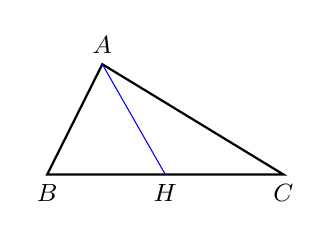
\begin{tikzpicture}[scale=1,font=\small]
\usetikzlibrary{calc}

\begin{scope}

\coordinate (b) at (0,0);
\coordinate (a) at (0.7,1.4);
\coordinate (c) at (3,0);

\draw[thick] (b) node[below] {$B$} -- (c) node[below] {$C$} -- (a) node[above] {$A$} -- cycle;

\coordinate (h) at ($(b)!0.5!(c)$);

\draw[blue] (h) node[black,below] {$H$} -- (a); % mediana
\end{scope}

\end{tikzpicture}

\end{minipage}
\end{esercizio}

% figura

\begin{esercizio}[Prove invalsi 2003]
\label{ese:2.100}
Da un triangolo equilatero $MNO$ di lato 6~cm viene tagliato via un triangolo equilatero di vertice in $O$ e lato 2~cm. Il perimetro del quadrilatero rimanente è \ldots
\begin{multicols}{5}
\begin{enumeratea}
\item 12~cm;
\item 14~cm;
\item 16~cm;
\item 18~cm;
\item 20~cm.
\end{enumeratea}
\end{multicols}
\end{esercizio}


%\cleardoublepage